% 第5章第6节：内积空间（内积与内积空间、Gram矩阵、子空间之间的正交、标准正交基的定义和性质、标准正交基的构建、伴随、完备性与Hilbert空间）。

\section{内积空间}
\label{sec:ls-inner-product-spaces}

上一节用范数度量大小，但范数不给出角度：一般范数下谈不上两个方向是否垂直，向子空间的最近点也可能不唯一（示例~\ref{ex:ls-linf-nonunique-nearest}）。第~\ref{chap:linear-operations}章在$\mathbb R^d$上定义了欧氏内积，并把它的三条基本性质取作内积的公理（定义~\ref{def:linear-algebra-inner-product}）。本节把内积搬到一般线性空间。

本节依次回答以下问题：一般空间上的内积怎样规定，由公理能推出哪些关于长度与夹角的结论；一组向量的两两内积怎样一次记录，选基以后内积怎样计算；一个向量怎样拆成落在子空间里的部分和与整个子空间垂直的部分，矩阵的四个基本子空间之间有怎样的垂直关系；什么样的基最便于计算，又怎样从任意一组基造出这样的基；对偶空间中的读取怎样借内积写成向量，线性映射怎样在配对中从一侧搬到另一侧；内积诱导的范数在什么情况下完备。前几个问题建立有限维内积空间的几何与计算工具；读取与伴随的问题把第~\ref{sec:ls-dual-spaces}节的对偶映射与内积联系起来；最后一个问题把第~\ref{sec:ls-banach-spaces}节的完备性用于内积空间，引出Hilbert空间，为无限维的函数空间作准备。

\subsection{内积与内积空间}
\label{sec:ls-inner-product-definition}

本小节只用内积的公理推出长度、夹角及相关不等式，说明内积空间都是赋范空间，并指出并非每个范数都来自内积。

\paragraph{一般线性空间上的内积}
内积的三条公理只用到加法与数乘，因此可以直接搬到一般线性空间上。
\begin{definition}[内积空间]
\label{def:functional-inner-product-space}
设$V$是实线性空间。映射$\langle\cdot,\cdot\rangle:V\times V\to\mathbb R$若对任意$\bm x,\bm y,\bm z\in V$与$a,b\in\mathbb R$满足
\begin{enumerate}
 \item 双线性：$\langle a\bm x+b\bm y,\bm z\rangle=a\langle\bm x,\bm z\rangle+b\langle\bm y,\bm z\rangle$，且$\langle\bm z,a\bm x+b\bm y\rangle=a\langle\bm z,\bm x\rangle+b\langle\bm z,\bm y\rangle$；
 \item 对称性：$\langle\bm x,\bm y\rangle=\langle\bm y,\bm x\rangle$；
 \item 正定性：$\langle\bm x,\bm x\rangle\geq0$，且$\langle\bm x,\bm x\rangle=0$当且仅当$\bm x=\bm0$，
\end{enumerate}
就称为$V$上的内积；配备内积的线性空间$(V,\langle\cdot,\cdot\rangle)$称为\term{内积空间}（inner-product space）。
\end{definition}
标准内积之外，一般空间上可以有各种内积。下面在$P_1$上规定一个只看两点取值的内积，后面的算例会反复用到它。
\begin{example}[只看两点取值的内积]
\label{ex:ls-two-point-inner-product}
给定：$P_1$上的规则$\langle f,g\rangle=f(0)g(0)+f(1)g(1)$。

验证：右端对$f$与对$g$分别是线性的，交换$f,g$也不改变右端，所以双线性与对称性成立。$\langle f,f\rangle=f(0)^2+f(1)^2\geq0$；若它为零，则$f(0)=f(1)=0$，对$f=a+bt$即$a=0$、$a+b=0$，故$f=0$，正定性也成立。

结论：这一规则是$P_1$上的内积。它只看函数在$t=0,1$两点的取值，与系数向量$(a,b)^\top$的欧氏内积不同：例如$\langle1,t\rangle=1\cdot0+1\cdot1=1$，而$1$与$t$的系数向量$(1,0)^\top$、$(0,1)^\top$的欧氏内积为零。
\end{example}

\paragraph{其他内积运算}
\phantomsection
\label{sec:ls-weighted-inner-products}
即使在$\mathbb R^d$上，标准内积也不是唯一的选择。各坐标的单位或重要性不同时，可以给不同方向不同的权重：取对称正定矩阵$\bm M$（第~\ref{sec:prelim-common-matrices}节），规定
\begin{equation}
 \langle\bm x,\bm y\rangle_{\bm M}=\bm x^\top\bm M\bm y,
 \qquad
 d_{\bm M}(\bm x,\bm y)=\lVert\bm x-\bm y\rVert_{\bm M}=\sqrt{(\bm x-\bm y)^\top\bm M(\bm x-\bm y)}.
 \label{eq:linear-algebra-mahalanobis-pseudodistance}
\end{equation}
双线性来自矩阵乘法的分配律，对称性来自$\bm M^\top=\bm M$，正定性就是$\bm M$的正定，所以它满足内积的三条公理，称为加权内积，$d_{\bm M}$是它给出的距离。统计中取$\bm M$为协方差矩阵的逆，得到的就是Mahalanobis距离。下面看权重怎样改变同一个点的长度。
\begin{example}[加权内积下的长度]
\label{ex:ls-weighted-length}
给定：$\bm M=\operatorname{diag}(4,1)$与$\bm x=(1,1)^\top$。

计算：$\langle\bm x,\bm y\rangle_{\bm M}=4x_1y_1+x_2y_2$，所以$\lVert\bm x\rVert_{\bm M}^2=4\cdot1+1\cdot1=5$；欧氏长度的平方则为$1+1=2$。

结论：同一个点的加权长度是$\sqrt5$，欧氏长度是$\sqrt2$；权重放大了第一个坐标的作用。
\end{example}
第~\ref{sec:ls-gram-psd}节将看到，选定基以后，任一内积在坐标下都是这种形式。下面的结论只用到内积公理，对标准内积、加权内积和示例~\ref{ex:ls-two-point-inner-product}中的内积同样成立。

\paragraph{长度与勾股定理}
与$\mathbb R^d$中一样，内积给出长度$\lVert\bm v\rVert=\sqrt{\langle\bm v,\bm v\rangle}$；$\langle\bm x,\bm y\rangle=0$时称$\bm x,\bm y$正交。正交的两个向量满足勾股定理：展开$\lVert\bm x+\bm y\rVert^2=\lVert\bm x\rVert^2+2\langle\bm x,\bm y\rangle+\lVert\bm y\rVert^2$，交叉项为零，得$\lVert\bm x+\bm y\rVert^2=\lVert\bm x\rVert^2+\lVert\bm y\rVert^2$。

\paragraph{Cauchy--Schwarz不等式}
平面上两个非零向量的夹角$\theta$满足
\[
 \langle\bm x,\bm y\rangle=\lVert\bm x\rVert\,\lVert\bm y\rVert\cos\theta.
\]
要在一般内积空间中反过来用这个关系定义夹角，须先保证内积除以两个长度之积以后总落在$[-1,1]$中。
\begin{theorem}[Cauchy--Schwarz不等式]
\label{thm:linear-algebra-cauchy-schwarz}
对任一内积及其长度，任意向量$\bm x,\bm y$满足
\begin{equation}
 |\langle\bm x,\bm y\rangle|\leq\lVert\bm x\rVert\,\lVert\bm y\rVert,
 \label{eq:prelim-cauchy-schwarz}
\end{equation}
等号成立当且仅当其中一个向量是另一个向量的实数倍。
\end{theorem}
\begin{proof}
$\bm y=\bm0$时两边都为零。否则对任意实数$s$，向量$\bm x-s\bm y$的长度平方非负；按内积的对称性与双线性展开，
\[
 0\leq\lVert\bm x-s\bm y\rVert^2
 =\lVert\bm x\rVert^2-2s\langle\bm x,\bm y\rangle+s^2\lVert\bm y\rVert^2.
\]
右侧是$s$的二次函数，二次项系数为正，取顶点$s=\langle\bm x,\bm y\rangle/\lVert\bm y\rVert^2$时最小，此时右侧化为$\lVert\bm x\rVert^2-\langle\bm x,\bm y\rangle^2/\lVert\bm y\rVert^2$。它非负，两边乘以$\lVert\bm y\rVert^2$再开平方，即得不等式。$\bm y\neq\bm0$时，等号成立当且仅当对这个$s$有$\bm x-s\bm y=\bm0$，即$\bm x$是$\bm y$的实数倍；连同$\bm y=\bm0$的情形即得等号条件。
\end{proof}
证明只用了内积的三条公理，所以不等式对每一种内积都成立。在$\mathbb R^d$的标准内积下，它就是$p=q=2$的Hölder不等式（定理~\ref{thm:linear-algebra-holder}）；对Frobenius内积，它给出$|\langle\bm A,\bm B\rangle_{\mathrm F}|\leq\lVert\bm A\rVert_{\mathrm F}\lVert\bm B\rVert_{\mathrm F}$。

\paragraph{三角不等式}
内积给出的长度是否满足定义~\ref{def:ls-normed-space}中范数的三条要求？正定性直接来自内积的正定性，齐次性来自$\langle c\bm x,c\bm x\rangle=c^2\langle\bm x,\bm x\rangle$；需要证明的是三角不等式，Cauchy--Schwarz不等式正好控制展开式中的交叉项。
\begin{theorem}[内积诱导长度的三角不等式]
\label{thm:ls-inner-product-triangle}
设$V$是内积空间，$\lVert\bm v\rVert=\sqrt{\langle\bm v,\bm v\rangle}$，则对任意$\bm x,\bm y\in V$，
\[
 \lVert\bm x+\bm y\rVert\leq\lVert\bm x\rVert+\lVert\bm y\rVert,
\]
等号成立当且仅当其中一个向量是另一个向量的非负实数倍。
\end{theorem}
\begin{proof}
按双线性与对称性展开平方，再对交叉项用$\langle\bm x,\bm y\rangle\leq|\langle\bm x,\bm y\rangle|$与Cauchy--Schwarz不等式~\eqref{eq:prelim-cauchy-schwarz}：
\[
 \lVert\bm x+\bm y\rVert^2
 =\lVert\bm x\rVert^2+2\langle\bm x,\bm y\rangle+\lVert\bm y\rVert^2
 \leq\lVert\bm x\rVert^2+2\lVert\bm x\rVert\lVert\bm y\rVert+\lVert\bm y\rVert^2
 =(\lVert\bm x\rVert+\lVert\bm y\rVert)^2.
\]
两边都非负，开平方即得不等式。等号成立当且仅当$\langle\bm x,\bm y\rangle=\lVert\bm x\rVert\,\lVert\bm y\rVert$。若$\bm y=\bm0$，结论显然；若$\bm y\neq\bm0$，由Cauchy--Schwarz不等式的等号条件，$\bm x=s\bm y$，代入得$s\lVert\bm y\rVert^2=|s|\,\lVert\bm y\rVert^2$，即$s\geq0$。反过来，$\bm x=s\bm y$且$s\geq0$时两侧都等于$(1+s)\lVert\bm y\rVert$。
\end{proof}
于是内积给出的长度满足范数的三条要求，每个内积空间都是赋范空间，第~\ref{sec:ls-normed-spaces}节关于收敛与完备性的讨论都适用于它。

\paragraph{夹角}
由Cauchy--Schwarz不等式，非零向量的夹角$\theta\in[0,\pi]$可以由
\[
 \cos\theta=\frac{\langle\bm x,\bm y\rangle}{\lVert\bm x\rVert\,\lVert\bm y\rVert}
 =\left\langle\frac{\bm x}{\lVert\bm x\rVert},\frac{\bm y}{\lVert\bm y\rVert}\right\rangle
\]
定义。第二种写法说明，夹角只比较方向：先把两个向量各自归一化为单位向量，再取内积；$\bm x$与$c\bm x$（$c>0$）给出同一个方向。正交恰好对应$\theta=\pi/2$，这就是把正交称为垂直的理由；等号条件说明$\cos\theta=\pm1$恰好对应两个向量共线。夹角要求长度来自同一个内积，一边用$\ell_2$、一边用$\ell_1$计量长度时，比值没有几何意义。

回到第~\ref{chap:linear-operations}章两个特征的取值向量，看它们的夹角。
\begin{example}[贯穿例两列的夹角]
\label{ex:ls-nearly-collinear-angle}
给定：$\bm c_1=(1,1,1)^\top$与$\bm c_2=(1,1+\varepsilon,1-\varepsilon)^\top$，取欧氏内积。

计算：$\langle\bm c_1,\bm c_2\rangle=1+(1+\varepsilon)+(1-\varepsilon)=3$，$\lVert\bm c_1\rVert_2^2=3$，$\lVert\bm c_2\rVert_2^2=1+(1+\varepsilon)^2+(1-\varepsilon)^2=3+2\varepsilon^2$，所以
\begin{equation}
 \cos\theta_\varepsilon=\frac{3}{\sqrt3\,\sqrt{3+2\varepsilon^2}}
 =\frac{1}{\sqrt{1+2\varepsilon^2/3}}\longrightarrow1\qquad(\varepsilon\to0).
 \label{eq:linear-algebra-nearly-collinear-angle}
\end{equation}
$\varepsilon=0.1$时$\cos\theta_\varepsilon\approx0.9967$，夹角约$4.7^\circ$；$\varepsilon=0.01$时$\cos\theta_\varepsilon\approx0.99997$，夹角不到$0.5^\circ$。

结论：$\varepsilon\to0$时两列的夹角趋于零；两个向量不重合，却几乎同向。
\end{example}
两个向量不重合却几乎同向，称为\term{近共线}（nearly collinear）。“近”指作为$\mathbb R^3$中向量的两列夹角很小，不是说各个样本点彼此接近。夹角也依赖所用的内积，换一种内积，同两个向量的夹角会改变。

夹角要求长度来自内积，而并非每个范数都来自内积。第~\ref{sec:ls-norms-distances}节对欧氏范数推出的平行四边形恒等式~\eqref{eq:functional-parallelogram-identity}只用到双线性与对称性，所以对每个内积诱导的范数同样成立；$\ell_1$与$\ell_\infty$范数不满足它，因而不来自任何内积，也就谈不上由它们定义夹角。还可以证明，满足平行四边形恒等式的范数都来自内积，可用极化公式$\langle\bm x,\bm y\rangle=(\lVert\bm x+\bm y\rVert^2-\lVert\bm x-\bm y\rVert^2)/4$恢复配对，这里不展开。内积比范数多出的正是角度与正交。

\subsection{Gram矩阵}
\label{sec:ls-gram-psd}

加权内积由一个正定矩阵给出。反过来看，一组向量的全部两两内积也排成一个对称矩阵。本小节说明，这样的矩阵恰好是全部半正定矩阵，从中可以读出这组向量是否线性无关、是否两两正交；最后用基的Gram矩阵写出一般内积空间在坐标下的计算公式。

\paragraph{Gram矩阵}
\phantomsection
\label{sec:ls-gram-orthogonality}
正交是两个向量之间的关系。一组向量$\bm b_1,\ldots,\bm b_r$之间有$r^2$个配对值，怎样一次记录它们，并从中读出这组向量是否两两正交、某个线性组合会不会退化为零？
\begin{definition}[有限向量族的Gram矩阵]
\label{def:linear-algebra-gram-matrix}
设$\bm b_1,\ldots,\bm b_r$是内积空间$V$中的向量。以$g_{i,j}=\langle\bm b_i,\bm b_j\rangle$为元素的$r$阶矩阵$\bm G$称为它们的\term{Gram矩阵}（Gram matrix）。在$\mathbb R^m$中，若$\bm B$以这些向量为列，则欧氏内积下$\bm G=\bm B^\top\bm B$，加权内积$\langle\cdot,\cdot\rangle_{\bm M}$下$\bm G=\bm B^\top\bm M\bm B$。
\end{definition}
矩阵形式来自乘积的元素公式：$(\bm B^\top\bm B)_{i,j}$是$\bm B^\top$的第$i$行（即$\bm b_i^\top$）与$\bm B$的第$j$列相乘。由内积的对称性，$\bm G$是对称矩阵。

对任意系数向量$\bm a\in\mathbb R^r$，按双线性展开得
\[
 \bm a^\top\bm G\bm a=\sum_{i,j}a_ia_j\langle\bm b_i,\bm b_j\rangle=\Bigl\lVert\sum_j a_j\bm b_j\Bigr\rVert^2\geq0,
\]
所以Gram矩阵半正定。它正定，当且仅当只有全零系数使线性组合$\sum_ja_j\bm b_j$为零，即这组向量线性无关（第~\ref{sec:ls-linear-dependence}节）：组合为零时平方长度为零，组合非零时平方长度为正。

正定的Gram矩阵可逆：若$\bm G\bm a=\bm0$，则$\bm a^\top\bm G\bm a=0$，从而$\bm a=\bm0$，零空间为零（第~\ref{sec:ls-injective-surjective-invertible}节）。正交性也写在Gram矩阵里：$\bm G$是对角矩阵恰好表示这组向量两两正交，$\bm G=\bm I_r$则表示它们两两正交且长度都为$1$。图~\ref{fig:ls-gram-matrix-coefficients}把两条向量的两两内积排成数表。
\begin{figure}[!htb]
  \centering
  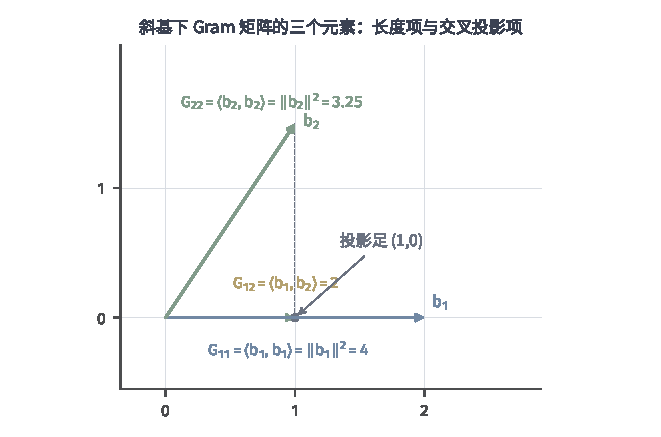
\includegraphics[width=112mm]{figures/01-mathematical-preliminaries-upper/02-linear-spaces/matplotlib/ls-gram-matrix-coefficients/ls-gram-matrix-coefficients.pdf}
  \caption{Gram矩阵把一组基向量的两两内积排成数表。左：平面上两条不垂直的基向量$\bm b_1,\bm b_2$及其夹角；右：$G_{i,j}=\langle\bm b_i,\bm b_j\rangle$构成的$2\times2$Gram矩阵，对角元为各向量长度平方，非对角元为夹角投影。基越接近正交，非对角元越接近零；两向量共线时，某个非零组合的平方长度为零，Gram矩阵不再正定。向量与矩阵均为解析教学例。}
  \label{fig:ls-gram-matrix-coefficients}
\end{figure}

近共线在Gram矩阵上怎样表现？
\begin{example}[近共线两列的Gram矩阵]
\label{ex:ls-nearly-collinear-gram}
给定：贯穿例的两列$\bm c_1,\bm c_2$，取欧氏内积。

计算：由示例~\ref{ex:ls-nearly-collinear-angle}中的三个内积，
\[
 \bm G=\bm X_\varepsilon^\top\bm X_\varepsilon=\begin{bmatrix}3&3\\3&3+2\varepsilon^2\end{bmatrix},
 \qquad
 \bm a^\top\bm G\bm a=3(a_1+a_2)^2+2\varepsilon^2a_2^2 .
\]
$\varepsilon\neq0$时，二次型只在$a_1=a_2=0$时为零，所以$\bm G$正定。取$\bm a=(1,-1)^\top$，二次型只有$2\varepsilon^2$；对应的组合$\bm c_1-\bm c_2=-\varepsilon\bm q$确实很短。

结论：$\bm G$正定，与两列线性无关一致；但存在系数使二次型接近零。近共线在Gram矩阵上表现为“正定但几乎退化”。
\end{example}

\paragraph{Gram因子定理}
Gram矩阵总是半正定的。反过来，每个半正定矩阵是否都是某组向量的Gram矩阵？关键是把半正定矩阵写成欧氏平方和，这一分解也说明加权配对不必当作新的几何。
\begin{theorem}[半正定矩阵的配方因子]
\label{thm:ls-gram-factor}
设$\bm M\in\mathbb R^{r\times r}$对称半正定，则存在$\bm L\in\mathbb R^{r\times r}$使$\bm M=\bm L^\top\bm L$；若$\bm M$正定，可取$\bm L$可逆。
\end{theorem}
\begin{proof}
对$r$归纳。$r=1$时$\bm M=(m_{1,1})$且$m_{1,1}\geq0$，取$\bm L=(\sqrt{m_{1,1}})$即可。

设$r>1$。若所有对角元都为零，任取$i\neq j$，把$\bm x=\bm e_i+t\bm e_j$代入半正定性：
\[
 0\leq\bm x^\top\bm M\bm x=m_{i,i}+2t\,m_{i,j}+t^2m_{j,j}=2t\,m_{i,j},
\]
对正负$t$同时成立迫使$m_{i,j}=0$，于是$\bm M=\bm0$，取$\bm L=\bm0$。

否则存在正的对角元。取一个置换矩阵$\bm P$把它换到首位（行列同步交换）；$\bm P$的各列是互不相同的标准坐标向量，所以$\bm P^\top\bm P=\bm P\bm P^\top=\bm I$。记
\[
 \widetilde{\bm M}=\bm P\bm M\bm P^\top
 =\begin{bmatrix}a&\bm b^\top\\ \bm b&\bm C\end{bmatrix},\qquad a>0.
\]
$\widetilde{\bm M}$仍对称半正定，因为$\bm x^\top\widetilde{\bm M}\bm x=(\bm P^\top\bm x)^\top\bm M(\bm P^\top\bm x)\geq0$。对第一个变量配方：令$\bm x=(-\bm b^\top\bm u/a,\bm u)$，展开得$\bm x^\top\widetilde{\bm M}\bm x=\bm u^\top(\bm C-\bm b\bm b^\top/a)\bm u\geq0$，故余项$\bm M'=\bm C-\bm b\bm b^\top/a$仍半正定。由归纳假设$\bm M'=\bm L'^\top\bm L'$，取上三角因子
\[
 \widetilde{\bm L}=\begin{bmatrix}\sqrt a&\bm b^\top/\sqrt a\\ \bm0&\bm L'\end{bmatrix},
\]
按分块乘法直接相乘得
\[
 \widetilde{\bm L}^\top\widetilde{\bm L}
 =\begin{bmatrix}a&\bm b^\top\\ \bm b&\bm b\bm b^\top/a+\bm L'^\top\bm L'\end{bmatrix}
 =\widetilde{\bm M}.
\]
换回原矩阵：$\bm M=\bm P^\top\widetilde{\bm M}\bm P=(\widetilde{\bm L}\bm P)^\top(\widetilde{\bm L}\bm P)$，取$\bm L=\widetilde{\bm L}\bm P$即可。

正定时$\bm M'$也正定（上述$\bm x$在$\bm u\neq\bm0$时非零），归纳得$\bm L'$可逆。分块上三角矩阵$\widetilde{\bm L}$的对角块$\sqrt a$与$\bm L'$都可逆，按分块乘法可以直接验证
\[
 \begin{bmatrix}1/\sqrt a&-\bm b^\top\bm L'^{-1}/a\\ \bm0&\bm L'^{-1}\end{bmatrix}
\]
是它的逆，于是$\bm L=\widetilde{\bm L}\bm P$作为可逆矩阵的乘积仍可逆。
\end{proof}
下面对一个二阶正定矩阵按证明的步骤求出因子。
\begin{example}[二阶正定矩阵的配方因子]
\label{ex:ls-gram-factor-two-by-two}
给定：$\bm M=\left[\begin{smallmatrix}4&2\\2&2\end{smallmatrix}\right]$。

计算：首个对角元$a=4>0$，不需要置换；$\bm b=(2)$，余项$\bm M'=2-2^2/4=1$，取$\bm L'=(1)$。按证明中的分块形式，
\[
 \bm L=\begin{bmatrix}\sqrt a&\bm b^\top/\sqrt a\\ 0&\bm L'\end{bmatrix}=\begin{bmatrix}2&1\\0&1\end{bmatrix}.
\]
直接验证：$\bm L^\top\bm L=\left[\begin{smallmatrix}2&0\\1&1\end{smallmatrix}\right]\left[\begin{smallmatrix}2&1\\0&1\end{smallmatrix}\right]=\left[\begin{smallmatrix}4&2\\2&2\end{smallmatrix}\right]=\bm M$。相应地，
\[
 \bm x^\top\bm M\bm x=4x_1^2+4x_1x_2+2x_2^2=(2x_1+x_2)^2+x_2^2 .
\]

结论：$\bm M=\bm L^\top\bm L$，且$\bm L$可逆；二次型被写成两个平方之和。
\end{example}
于是正定矩阵给出的加权长度可写成$\lVert\bm x\rVert_{\bm M}=\lVert\bm L\bm x\rVert_2$：加权内积只是把$\bm x$换成新坐标$\bm L\bm x$再量欧氏长度。证明中的配方步骤就是第~\ref{sec:ls-exact-linear-equations}节Cholesky分解的雏形。

\paragraph{半正定矩阵与Gram矩阵}
Gram矩阵总是半正定的；反过来，每个半正定矩阵都是某组向量的Gram矩阵。由定理~\ref{thm:ls-gram-factor}，半正定的$\bm M$可写成$\bm M=\bm L^\top\bm L$，记$\bm l_i$为$\bm L$的第$i$列，则$m_{i,j}=\bm l_i^\top\bm l_j=\langle\bm l_i,\bm l_j\rangle$，$\bm M$正是$\bm l_1,\ldots,\bm l_r$在欧氏内积下的Gram矩阵。所以“半正定”与“是一组向量的两两内积”说的是同一件事，判断一个矩阵半正定，可以去找这样一组向量。

这一观点给出一个关于逐元素乘积（第~\ref{sec:ls-hadamard-product}节）的结论：两个半正定矩阵的逐元素乘积仍半正定吗？设$\bm A,\bm B$均为$n$阶半正定矩阵。由定理~\ref{thm:ls-gram-factor}，$\bm A=\bm U^\top\bm U$、$\bm B=\bm V^\top\bm V$；记$\bm u_i,\bm v_i$分别为$\bm U,\bm V$的第$i$列，则$A_{i,k}=\langle\bm u_i,\bm u_k\rangle$、$B_{i,k}=\langle\bm v_i,\bm v_k\rangle$。考虑二阶数组$\bm u_1\otimes\bm v_1,\ldots,\bm u_n\otimes\bm v_n$，由Frobenius内积下张量积配对的分离性（第~\ref{sec:ls-tensor-operation-properties}节），它们的Gram矩阵为
\[
 \langle\bm u_i\otimes\bm v_i,\bm u_k\otimes\bm v_k\rangle_{\mathrm F}
 =\langle\bm u_i,\bm u_k\rangle\langle\bm v_i,\bm v_k\rangle
 =A_{i,k}B_{i,k}.
\]
Gram矩阵恒半正定，故逐元素乘积$\bm A\odot\bm B$半正定，这就是\term{Schur乘积}定理（Schur product theorem）。下面用一个二阶例子核对。
\begin{example}[两个半正定矩阵的逐元素乘积]
\label{ex:ls-schur-product}
给定：$\bm A=\bm B=\left[\begin{smallmatrix}1&1\\1&2\end{smallmatrix}\right]$。

计算：$\bm A$的二次型为$x_1^2+2x_1x_2+2x_2^2=(x_1+x_2)^2+x_2^2\geq0$，所以$\bm A$半正定。逐元素乘积及其二次型为
\[
 \bm A\odot\bm B=\begin{bmatrix}1&1\\1&4\end{bmatrix},
 \qquad
 x_1^2+2x_1x_2+4x_2^2=(x_1+x_2)^2+3x_2^2\geq0 .
\]

结论：$\bm A\odot\bm B$仍半正定，与Schur乘积定理一致。
\end{example}
核方法中两个核矩阵的逐元素乘积仍是合法的核矩阵，依据就是这一定理。

\paragraph{坐标下的内积}
选定基以后，一般内积空间上的内积也由一张矩阵完全确定，这张矩阵就是基的Gram矩阵。设$\mathcal B=(\bm b_1,\ldots,\bm b_d)$是$V$的基，$\bm G$是它的Gram矩阵。对$\bm v=\sum_ix_i\bm b_i$、$\bm w=\sum_jy_j\bm b_j$，按双线性展开得
\[
 \langle\bm v,\bm w\rangle=\sum_{i,j}x_iy_j\langle\bm b_i,\bm b_j\rangle=[\bm v]_{\mathcal B}^\top\,\bm G\,[\bm w]_{\mathcal B}.
\]
基线性无关，所以$\bm G$对称正定：在坐标下，任一内积都是以$\bm G$为权重的加权内积。特别地，$\mathbb R^d$上的任一内积在标准基下都是$\bm x^\top\bm G\bm y$，其中$g_{i,j}=\langle\bm e_i,\bm e_j\rangle$；反过来，每个对称正定矩阵都给出一个加权内积。所以$\mathbb R^d$上的内积与$d$阶对称正定矩阵一一对应，欧氏内积对应$\bm I$。下面用示例~\ref{ex:ls-two-point-inner-product}的内积核对坐标公式。
\begin{example}[两点内积的坐标计算]
\label{ex:ls-two-point-inner-product-coordinates}
给定：示例~\ref{ex:ls-two-point-inner-product}中$P_1$上的内积$\langle f,g\rangle=f(0)g(0)+f(1)g(1)$，基$(1,t)$，以及$f=1+t$、$g=1-2t$。

计算：由$\langle1,1\rangle=1\cdot1+1\cdot1=2$、$\langle1,t\rangle=1\cdot0+1\cdot1=1$、$\langle t,t\rangle=0\cdot0+1\cdot1=1$，基的Gram矩阵为
\[
 \bm G=\begin{bmatrix}2&1\\1&1\end{bmatrix}.
\]
按定义，$f$在$t=0,1$处取值$1,2$，$g$取值$1,-1$，所以$\langle f,g\rangle=1\cdot1+2\cdot(-1)=-1$。按坐标，$[f]=(1,1)^\top$、$[g]=(1,-2)^\top$，
\[
 (1,1)\,\bm G\begin{bmatrix}1\\-2\end{bmatrix}=(3,2)\begin{bmatrix}1\\-2\end{bmatrix}=-1 .
\]

结论：两种算法给出同一个内积值$-1$。
\end{example}
若基两两正交且长度为$1$，则$\bm G=\bm I$，内积在坐标下就是欧氏内积；这样的基是第~\ref{sec:ls-orthonormal-bases}节的主题。

\subsection{子空间之间的正交}
\label{sec:ls-orthogonality}

Gram矩阵记录的是一组向量两两之间是否正交。本小节把正交推广为一个向量与整个子空间的正交，得到由内积唯一确定的补空间，并据此证明四个基本子空间之间的垂直关系。

\paragraph{正交补}
第~\ref{sec:ls-direct-sum}节说明，一个子空间的补空间一般不唯一。有了内积，是否存在一个由“垂直”唯一确定的补空间？设$U$是有限维内积空间$V$的子空间，与$U$中每个向量都正交的向量组成的集合
\[
 U^\perp=\{\bm r\in V:\langle\bm u,\bm r\rangle=0,\ \forall\bm u\in U\}
\]
称为$U$的\term{正交补}（orthogonal complement）。由内积的双线性，$U^\perp$对线性组合封闭，是子空间。要检查$\bm r\in U^\perp$，只需检查它与$U$的一组基逐个正交，因为与基向量都正交的向量与基向量的每个组合也正交。

\paragraph{正交直和}
正交补确实是一个补空间，而且分解可以由Gram矩阵算出。
\begin{lemma}[正交直和]
\label{lem:ls-orthogonal-decomposition}
设$U$是有限维内积空间$V$的子空间，则每个$\bm x\in V$唯一分解为$\bm x=\bm u+\bm r$，其中$\bm u\in U$、$\bm r\in U^\perp$；即$V=U\oplus U^\perp$。
\end{lemma}
\begin{proof}
取$U$的一组基$\bm b_1,\ldots,\bm b_r$，它线性无关，所以Gram矩阵$\bm G$正定，从而可逆。对任意$\bm x$，令$\bm u=\sum_j a_j\bm b_j$，并要求$\bm r=\bm x-\bm u$与每个$\bm b_i$正交，得到系数方程
\[
 \sum_j g_{i,j}a_j=\langle\bm b_i,\bm x\rangle,\qquad i=1,\ldots,r,
\]
即$\bm G\bm a=(\langle\bm b_i,\bm x\rangle)_i$。可逆的$\bm G$保证系数唯一解出，残差$\bm r$与全部基向量正交，因而落在$U^\perp$。

若$\bm x=\bm u+\bm r=\bm u'+\bm r'$是两种分解，则$\bm u-\bm u'=\bm r'-\bm r$同时属于$U$与$U^\perp$，与自身正交，长度为零，故两种分解相同。
\end{proof}
所以正交补是$U$的一个补空间，并且由内积唯一确定，称$V=U\oplus U^\perp$为正交直和；由维数公式，$\dim U^\perp=\dim V-\dim U$。下面在$\mathbb R^3$中做一次分解。
\begin{example}[向一条直线的正交分解]
\label{ex:ls-orthogonal-decomposition-line}
给定：$\mathbb R^3$取欧氏内积，$U=\operatorname{span}\{\bm c_1\}$，$\bm c_1=(1,1,1)^\top$，$\bm y=(1,1.1,0.9)^\top$。

计算：$U^\perp$由与$\bm c_1$正交的向量组成，即坐标和为零的平面。$U$只有一个基向量，Gram方程只有一个未知数：$\langle\bm c_1,\bm c_1\rangle a=\langle\bm c_1,\bm y\rangle$，即$3a=3$，所以$a=1$。于是
\[
 \bm u=\bm c_1=(1,1,1)^\top,
 \qquad
 \bm r=\bm y-\bm u=(0,0.1,-0.1)^\top,
\]
$\bm r$的坐标和为零，确实属于$U^\perp$。

结论：$\bm y=\bm u+\bm r$就是$\bm y$在正交直和$\mathbb R^3=U\oplus U^\perp$中的分解。
\end{example}
这里只证明正交分量存在且唯一；它就是$U$中离$\bm x$最近的点，这一判定与具体算法在第~\ref{sec:ls-subspace-nearest-points}节给出。

取两次正交补会回到原来的子空间：$(U^\perp)^\perp=U$。一方面，$U$中每个向量与$U^\perp$中每个向量正交，所以$U\subseteq(U^\perp)^\perp$；另一方面，对$U^\perp$用上面的维数关系，$\dim(U^\perp)^\perp=\dim V-\dim U^\perp=\dim U$。包含且同维，由第~\ref{sec:ls-dimension}节两者相等。

\paragraph{四个基本子空间的正交关系}
示例~\ref{ex:ls-rank-one-four-subspaces}显示，行空间的方向与零空间垂直，列空间的方向与左零空间垂直。现在在$\mathbb R^d$与$\mathbb R^m$上取欧氏内积，证明这对任何矩阵都成立。
\begin{theorem}[四个基本子空间的正交关系]
\label{thm:ls-four-subspaces-orthogonality}
设$\bm A\in\mathbb R^{m\times d}$，$\mathbb R^d$与$\mathbb R^m$取欧氏内积。则
\begin{equation}
 \operatorname{null}(\bm A)=\operatorname{range}(\bm A^\top)^\perp,\qquad
 \operatorname{null}(\bm A^\top)=\operatorname{range}(\bm A)^\perp,
 \label{eq:ls-four-subspaces-orthogonality}
\end{equation}
因而有正交直和
\begin{equation}
 \mathbb R^d=\operatorname{range}(\bm A^\top)\oplus\operatorname{null}(\bm A),\qquad
 \mathbb R^m=\operatorname{range}(\bm A)\oplus\operatorname{null}(\bm A^\top).
 \label{eq:ls-four-subspaces-decomposition}
\end{equation}
\end{theorem}
\begin{proof}
由转置的乘积规则（第~\ref{sec:ls-reshaping}节），对任意$\bm x\in\mathbb R^d$、$\bm y\in\mathbb R^m$，
\[
 \langle\bm A\bm x,\bm y\rangle=(\bm A\bm x)^\top\bm y=\bm x^\top(\bm A^\top\bm y)=\langle\bm x,\bm A^\top\bm y\rangle.
\]
$\bm y\in\operatorname{range}(\bm A)^\perp$意味着左端对一切$\bm x$为零，即右端对一切$\bm x$为零；取$\bm x=\bm A^\top\bm y$可见这当且仅当$\bm A^\top\bm y=\bm0$。所以$\operatorname{range}(\bm A)^\perp=\operatorname{null}(\bm A^\top)$。把$\bm A$换成$\bm A^\top$得$\operatorname{range}(\bm A^\top)^\perp=\operatorname{null}(\bm A)$。正交直和由引理~\ref{lem:ls-orthogonal-decomposition}得到。
\end{proof}
两边再取正交补，并用$(U^\perp)^\perp=U$，还得到$\operatorname{null}(\bm A)^\perp=\operatorname{range}(\bm A^\top)$、$\operatorname{null}(\bm A^\top)^\perp=\operatorname{range}(\bm A)$。于是输入空间分成两块互相垂直的部分：零空间是被$\bm A$消去的方向，行空间是真正影响输出的方向；输出空间也分成两块：列空间是可达的输出，左零空间是无论如何都到达不了的方向。

这一定理与第~\ref{sec:ls-kernel-image}节的维数关系相互印证。由正交直和与秩零度定理分别得到
\[
 d=\dim\operatorname{range}(\bm A^\top)+\dim\operatorname{null}(\bm A),\qquad
 d=\operatorname{rank}\bm A+\dim\operatorname{null}(\bm A).
\]
两式比较，又一次得到行秩等于列秩。示例~\ref{ex:ls-rank-one-four-subspaces}中逐项相乘再相加得零的观察，现在由定理得到了解释。

输出端的分解给出方程$\bm A\bm x=\bm b$有解的一个判据：$\bm b\in\operatorname{range}(\bm A)$当且仅当$\bm b$与左零空间中每个向量正交。第~\ref{chap:linear-equations-and-optimization}章判断方程是否有解时会用到这一点。

\subsection{标准正交基的定义和性质}
\label{sec:ls-orthonormal-bases}

正交直和的证明要解Gram方程$\bm G\bm a=(\langle\bm b_i,\bm x\rangle)_i$，坐标下的内积要乘Gram矩阵，示例~\ref{ex:ls-coordinate-instability}还显示，接近共线的基会把小的对象记成很大的系数。这些麻烦都来自基向量之间的相互干扰，即Gram矩阵的非对角元。本小节定义消除这种干扰的基，证明它确实是一组基，再依次给出它下的坐标、它们之间的换基，以及向子空间的正交分解。

\paragraph{标准正交基的定义}
一组向量$\bm q_1,\ldots,\bm q_r$若满足
\[
 \langle\bm q_i,\bm q_j\rangle=\delta_{i,j}=\begin{cases}1,&i=j,\\0,&i\neq j,\end{cases}
\]
即两两正交且长度都为$1$，就称为标准正交组；它的Gram矩阵是$\bm I_r$。张成子空间$U$的标准正交组称为$U$的\term{标准正交基}（orthonormal basis）；$U=V$时就是$V$的标准正交基。

在$\mathbb R^m$中取欧氏内积，把$r$个向量排成$\bm Q\in\mathbb R^{m\times r}$的各列，它们的Gram矩阵是$\bm Q^\top\bm Q$，所以标准正交的条件就是$\bm Q^\top\bm Q=\bm I_r$。$r=m$时$\bm Q$是第~\ref{sec:ls-orthogonal-matrices}节的正交矩阵；$r<m$时$\bm Q^\top\bm Q=\bm I_r$仍成立，但$\bm Q\bm Q^\top$的秩只有$r$，不等于$\bm I_m$，$\bm Q$只有左逆$\bm Q^\top$。

\paragraph{标准正交组构成基}
标准正交组总是线性无关。设$\sum_jc_j\bm q_j=\bm0$，两边与$\bm q_i$作内积，左边每一项$c_j\langle\bm q_j,\bm q_i\rangle$只在$j=i$时不为零，于是$c_i=0$；$i$任意，所以全部系数为零。同样的论证说明两两正交的非零向量组线性无关，只是最后一步改为由$c_i\langle\bm q_i,\bm q_i\rangle=0$与$\langle\bm q_i,\bm q_i\rangle>0$得$c_i=0$。因此标准正交组是它所张成子空间的一组基；$d$维内积空间中$d$个两两正交的单位向量个数等于维数，自动构成整个空间的标准正交基，不必另行验证张成。$\mathbb R^d$的标准基在欧氏内积下是标准正交基；$\bm q_1=(1,1)^\top/\sqrt2$、$\bm q_2=(1,-1)^\top/\sqrt2$是$\mathbb R^2$的另一组标准正交基。

\paragraph{标准正交基下的坐标}
在标准正交基下，坐标不必解方程。若$\bm v=\sum_jc_j\bm q_j$，两边与$\bm q_i$作内积，右边只剩$c_i$一项，所以
\begin{equation}
 \bm v=\sum_{j=1}^d\langle\bm v,\bm q_j\rangle\,\bm q_j.
 \label{eq:ls-orthonormal-expansion}
\end{equation}
每个系数只与自己的方向有关，增加或删去其他方向都不改变它。坐标下的内积变成欧氏内积：$\langle\bm v,\bm w\rangle=\sum_jc_jd_j$，其中$c_j,d_j$分别是$\bm v,\bm w$的坐标；特别地
\begin{equation}
 \lVert\bm v\rVert^2=\sum_{j=1}^d\langle\bm v,\bm q_j\rangle^2,
 \label{eq:ls-parseval}
\end{equation}
长度的平方等于各坐标的平方和，称为Parseval恒等式，是勾股定理在$d$个互相垂直方向上的推广。下面用平面上的一组标准正交基验证这两点。
\begin{example}[标准正交基下的坐标与Parseval恒等式]
\label{ex:ls-orthonormal-coordinates}
给定：$\mathbb R^2$的标准正交基$\bm q_1=(1,1)^\top/\sqrt2$、$\bm q_2=(1,-1)^\top/\sqrt2$，向量$\bm v=(3,1)^\top$。

计算：由式~\eqref{eq:ls-orthonormal-expansion}，坐标为$\langle\bm v,\bm q_1\rangle=4/\sqrt2=2\sqrt2$与$\langle\bm v,\bm q_2\rangle=2/\sqrt2=\sqrt2$，不必解方程。坐标的平方和为$8+2=10$，而$\lVert\bm v\rVert^2=3^2+1^2=10$。

结论：坐标由内积直接读出，平方和等于长度的平方。
\end{example}
在标准正交基下，坐标的大小如实反映对象的大小，近共线基下“小对象、大系数”的现象不会发生。

\paragraph{标准正交基之间的换基}
设$\mathcal B=(\bm b_1,\ldots,\bm b_d)$与$\mathcal C$都是$V$的标准正交基，换基矩阵$\bm S=\bm S_{\mathcal C\leftarrow\mathcal B}$的第$j$列是$\bm b_j$的$\mathcal C$坐标。在标准正交基$\mathcal C$下内积就是坐标的欧氏内积，所以$\bm S$的第$i$、$j$两列的欧氏内积等于$\langle\bm b_i,\bm b_j\rangle=\delta_{i,j}$，即$\bm S^\top\bm S=\bm I$：两组标准正交基之间的换基矩阵是正交矩阵。

于是反向换基只需转置，$\bm S^{-1}=\bm S^\top$，不会出现示例~\ref{ex:ls-nearly-collinear-change-of-basis}中除以小数$\varepsilon$的放大。例如从上面的$(\bm q_1,\bm q_2)$换到标准基，换基矩阵的两列就是$\bm q_1,\bm q_2$本身。对线性算子，若只在标准正交基之间换基，相似关系$\bm B=\bm P^{-1}\bm A\bm P$变成$\bm B=\bm P^\top\bm A\bm P$；第~\ref{chap:linear-analysis}章的谱定理正是要在这一受限的换基下化简对称矩阵。

\paragraph{向子空间的正交分解}
若$\bm q_1,\ldots,\bm q_r$是子空间$U$的标准正交基，第~\ref{sec:ls-orthogonality}节正交直和中的Gram方程变成$\bm a=(\langle\bm q_i,\bm x\rangle)_i$，分解直接写出：
\begin{equation}
 \bm x=\underbrace{\sum_{j=1}^r\langle\bm x,\bm q_j\rangle\bm q_j}_{\bm u\in U}+\underbrace{\Bigl(\bm x-\sum_{j=1}^r\langle\bm x,\bm q_j\rangle\bm q_j\Bigr)}_{\bm r\in U^\perp}.
 \label{eq:ls-orthonormal-projection}
\end{equation}
$\bm u$称为$\bm x$在$U$上的正交投影。$\bm u$与$\bm r$正交，由勾股定理$\lVert\bm x\rVert^2=\lVert\bm u\rVert^2+\lVert\bm r\rVert^2\geq\sum_{j=1}^r\langle\bm x,\bm q_j\rangle^2$：沿一部分标准正交方向读出的系数平方和不超过总长度的平方，等号恰在$\bm x\in U$时成立。下面用这一公式重算示例~\ref{ex:ls-orthogonal-decomposition-line}中的分解。
\begin{example}[用标准正交基重算正交分解]
\label{ex:ls-orthonormal-projection-line}
给定：$U=\operatorname{span}\{\bm q_1\}$，$\bm q_1=(1,1,1)^\top/\sqrt3$，$\bm y=(1,1.1,0.9)^\top$。

计算：$\langle\bm y,\bm q_1\rangle=3/\sqrt3=\sqrt3$，投影为$\sqrt3\,\bm q_1=(1,1,1)^\top$，余量为$(0,0.1,-0.1)^\top$，它与$\bm q_1$正交。

结论：结果与示例~\ref{ex:ls-orthogonal-decomposition-line}相同，但这里不需要解Gram方程。
\end{example}
下一小节构造标准正交基，靠的正是这一公式。

\subsection{标准正交基的构建}
\label{sec:ls-orthonormal-basis-construction}

标准正交基如此方便，它是否总存在？给定任意一组基，怎样把它改造成标准正交基？上一小节的正交分解给出了思路：依次处理基向量，从每个向量中扣除它在已经造好的方向上的分量，剩下的部分与这些方向都垂直，再把它缩放到单位长度。本小节先给出这一过程并证明它总能完成，再把它在$\mathbb R^m$中写成矩阵分解，最后处理各列线性相关的情形。

\subsubsection{Gram--Schmidt正交化}

这一过程称为\term{Gram--Schmidt正交化}（Gram--Schmidt orthogonalization），也称施密特正交化。设$\bm v_1,\ldots,\bm v_k$线性无关。令$\bm u_1=\bm v_1$、$\bm q_1=\bm u_1/\lVert\bm u_1\rVert$；对$j=2,\ldots,k$依次令
\begin{equation}
 \bm u_j=\bm v_j-\sum_{i=1}^{j-1}\langle\bm v_j,\bm q_i\rangle\bm q_i,
 \qquad
 \bm q_j=\frac{\bm u_j}{\lVert\bm u_j\rVert}.
 \label{eq:ls-gram-schmidt}
\end{equation}
按式~\eqref{eq:ls-orthonormal-projection}，$\bm u_j$正是$\bm v_j$在$\operatorname{span}\{\bm q_1,\ldots,\bm q_{j-1}\}$的正交补中的分量。
\begin{theorem}[Gram--Schmidt正交化]
\label{thm:ls-gram-schmidt}
上述过程中每个$\bm u_j\neq\bm0$，得到的$\bm q_1,\ldots,\bm q_k$两两正交、长度为$1$，并且对每个$j$都有$\operatorname{span}\{\bm q_1,\ldots,\bm q_j\}=\operatorname{span}\{\bm v_1,\ldots,\bm v_j\}$。
\end{theorem}
\begin{proof}
对$j$归纳。$j=1$时$\bm u_1=\bm v_1\neq\bm0$，结论成立。设结论对$j-1$成立。对$i<j$，由$\bm q_1,\ldots,\bm q_{j-1}$两两正交且长度为$1$，
\[
 \langle\bm u_j,\bm q_i\rangle=\langle\bm v_j,\bm q_i\rangle-\langle\bm v_j,\bm q_i\rangle\langle\bm q_i,\bm q_i\rangle=0,
\]
所以$\bm u_j$与前面的方向都正交。若$\bm u_j=\bm0$，则$\bm v_j$属于$\operatorname{span}\{\bm q_1,\ldots,\bm q_{j-1}\}=\operatorname{span}\{\bm v_1,\ldots,\bm v_{j-1}\}$，与线性无关矛盾；故$\bm u_j\neq\bm0$，$\bm q_j$有定义且长度为$1$。最后，$\bm q_j$是$\bm v_j$与$\bm q_1,\ldots,\bm q_{j-1}$的组合，因而属于$\operatorname{span}\{\bm v_1,\ldots,\bm v_j\}$；反过来由式~\eqref{eq:ls-gram-schmidt}，$\bm v_j=\lVert\bm u_j\rVert\bm q_j+\sum_{i<j}\langle\bm v_j,\bm q_i\rangle\bm q_i$属于$\operatorname{span}\{\bm q_1,\ldots,\bm q_j\}$。两个张成空间互相包含，因而相等。
\end{proof}
对有限维内积空间的任意一组基作Gram--Schmidt正交化，就得到一组标准正交基，所以\emph{每个有限维内积空间都有标准正交基}。若已有几个两两正交的单位向量，先把它们扩充成一组基，再从它们之后开始正交化：前面的向量在过程中保持不变，所以任何标准正交组都能扩充成标准正交基。张成空间逐段相等也有用处：前$j$个新方向与前$j$个旧方向张成同一个子空间，正交化只是在每一段内部换了一组更好用的基。

\paragraph{算例}
标准正交基依赖内积，换一个内积，同一组基正交化的结果也不同。下面在示例~\ref{ex:ls-two-point-inner-product}的内积下对基$(1,t)$作正交化；在这个内积下$\langle1,t\rangle=1\neq0$，两个基向量并不正交。
\begin{example}[两点内积下的Gram--Schmidt正交化]
\label{ex:ls-gram-schmidt-two-point}
给定：$P_1$上的内积$\langle f,g\rangle=f(0)g(0)+f(1)g(1)$，基$(1,t)$。

计算：第一步，归一化第一个基向量。$\lVert1\rVert^2=1^2+1^2=2$，所以
\[
 q_1=\frac1{\sqrt2}.
\]

第二步，从第二个基向量中扣除它在$q_1$上的分量。$\langle t,q_1\rangle=\bigl(0\cdot1+1\cdot1\bigr)/\sqrt2=1/\sqrt2$，所以
\[
 u_2=t-\langle t,q_1\rangle q_1=t-\frac1{\sqrt2}\cdot\frac1{\sqrt2}=t-\frac12.
\]

第三步，归一化。$u_2$在$t=0,1$处的取值为$-\tfrac12,\tfrac12$，所以$\lVert u_2\rVert^2=\tfrac14+\tfrac14=\tfrac12$，
\[
 q_2=\frac{u_2}{\lVert u_2\rVert}=\sqrt2\Bigl(t-\frac12\Bigr).
\]

第四步，核对。$q_1$在$t=0,1$处取值都是$\tfrac1{\sqrt2}$，$q_2$取值为$-\tfrac{\sqrt2}2,\tfrac{\sqrt2}2$，所以$\langle q_1,q_2\rangle=\tfrac1{\sqrt2}\cdot\bigl(-\tfrac{\sqrt2}2\bigr)+\tfrac1{\sqrt2}\cdot\tfrac{\sqrt2}2=0$，$\lVert q_2\rVert^2=\tfrac12+\tfrac12=1$。

第五步，用新基读坐标。$f=1+t$在$t=0,1$处取值为$1,2$，所以$\langle f,q_1\rangle=(1+2)/\sqrt2=3/\sqrt2$，$\langle f,q_2\rangle=1\cdot\bigl(-\tfrac{\sqrt2}2\bigr)+2\cdot\tfrac{\sqrt2}2=\tfrac{\sqrt2}2$。还原得$\tfrac3{\sqrt2}\cdot\tfrac1{\sqrt2}+\tfrac{\sqrt2}2\cdot\sqrt2(t-\tfrac12)=\tfrac32+t-\tfrac12=1+t$。Parseval恒等式也成立：$\lVert f\rVert^2=1^2+2^2=5$，而$\tfrac92+\tfrac12=5$。

结论：$q_1=1/\sqrt2$、$q_2=\sqrt2(t-\tfrac12)$是这一内积下$P_1$的标准正交基，$1+t$在其下的坐标为$(3/\sqrt2,\ \sqrt2/2)$。
\end{example}
正交化把$t$换成了$t-\tfrac12$。在系数向量的欧氏内积下，$1$与$t$的系数列$(1,0)^\top$、$(0,1)^\top$本来就正交；换了内积以后，却需要这一步。

\subsubsection{QR分解}

在$\mathbb R^m$中取欧氏内积，Gram--Schmidt正交化可以写成一个矩阵等式，它把一组列向量的方向与组合系数分开记录。设$\bm A\in\mathbb R^{m\times d}$的列$\bm a_1,\ldots,\bm a_d$线性无关，对它们作正交化（即取$\bm v_j=\bm a_j$）。把式~\eqref{eq:ls-gram-schmidt}反过来写，$\bm a_j=\lVert\bm u_j\rVert\bm q_j+\sum_{i<j}\langle\bm a_j,\bm q_i\rangle\bm q_i$，即每一列只用到前$j$个正交方向：
\[
 \bm a_j=\sum_{i\leq j}r_{i,j}\bm q_i,\qquad
 r_{i,j}=\langle\bm a_j,\bm q_i\rangle\ (i<j),\qquad r_{j,j}=\lVert\bm u_j\rVert>0 .
\]
把$\bm q_1,\ldots,\bm q_d$排成$\bm Q\in\mathbb R^{m\times d}$，把系数$r_{i,j}$排成$d$阶上三角矩阵$\bm R$（$i>j$时$r_{i,j}=0$），按矩阵乘积的列读法，各列的这些关系合写为经济型\term{QR分解}（QR factorization）
\begin{equation}
 \bm A=\bm Q\bm R,\qquad
 \bm Q^\top\bm Q=\bm I_d,\quad\bm R\text{ 上三角且对角元为正}.
 \label{eq:ls-qr-factorization}
\end{equation}
由定理~\ref{thm:ls-gram-schmidt}，$\bm Q$的列是列空间$\operatorname{range}(\bm A)$的标准正交基，$\bm R$的第$j$列记录$\bm a_j$在这组正交方向上的坐标；$\bm R$的对角元为正，所以$\bm R$可逆。图~\ref{fig:vol1-add-linear-qr-columns}给出最小的二维情形：保留第一条单位方向，从第二列减去它在第一方向上的分量，列空间不变，减去的部分记进$\bm R$。
\begin{figure}[!htb]
  \centering
  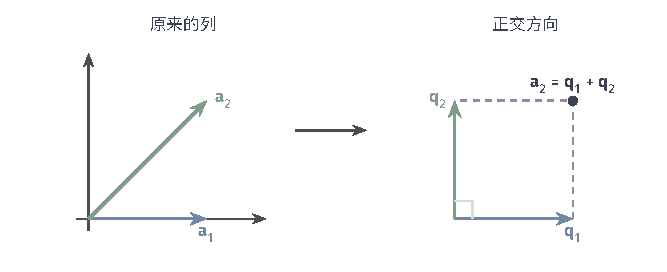
\includegraphics[width=112mm]{figures/01-mathematical-preliminaries-upper/02-linear-spaces/tikz/comprehension-additions/linear-qr-columns.pdf}
  \caption{QR把列的方向和组合系数分开。取$\bm a_1=(1,0)^\top$、$\bm a_2=(1,1)^\top$，
  正交化得到$\bm q_1=(1,0)^\top$、$\bm q_2=(0,1)^\top$，并有$\bm a_1=\bm q_1$、
  $\bm a_2=\bm q_1+\bm q_2$，故$\bm R=\left[\begin{smallmatrix}1&1\\0&1\end{smallmatrix}\right]$。
  虚线补出第二列的分量。}
  \label{fig:vol1-add-linear-qr-columns}
\end{figure}

这一分解的用处在于，涉及列空间的计算可以改在标准正交的$\bm Q$上进行，坐标由内积直接读出，不必再解Gram方程；第~\ref{chap:linear-equations-and-optimization}章解方程与最小二乘问题时正是这样使用它的。

\subsubsection{列相关时的处理}

定理~\ref{thm:ls-gram-schmidt}要求各列线性无关。若不满足，某一步会出现$\bm u_j=\bm0$：由式~\eqref{eq:ls-orthonormal-projection}，这恰好说明$\bm a_j$已在前面方向张成的空间中，没有带来新方向。这时不能对零向量归一化，应跳过这一列，只在$\bm R$中记下它的系数$\langle\bm a_j,\bm q_i\rangle$；跳过它不影响后续各列，因为张成的空间没有变。

全部处理完以后，留下的$\bm q$个数等于列空间的维数$r=\operatorname{rank}\bm A$，仍有$\bm A=\bm Q\bm R$，其中$\bm Q\in\mathbb R^{m\times r}$的列是列空间的标准正交基，$\bm R\in\mathbb R^{r\times d}$的各行从左到右第一个非零元的位置逐行右移；$r<d$时$\bm R$不是方阵，不能求逆。下面是最小的例子。
\begin{example}[列相关时跳过零余量]
\label{ex:ls-qr-dependent-columns}
给定：$\bm A=[\bm a_1\ \bm a_2]$，$\bm a_1=(1,0)^\top$、$\bm a_2=(2,0)^\top$。

计算：$\bm q_1=\bm a_1$。$\langle\bm a_2,\bm q_1\rangle=2$，扣除后$\bm u_2=\bm a_2-2\bm q_1=\bm0$，所以跳过$\bm a_2$，只在$\bm R$中记下系数$2$。于是$r=1$，
\[
 \bm Q=\begin{bmatrix}1\\0\end{bmatrix},\qquad
 \bm R=\begin{bmatrix}1&2\end{bmatrix},\qquad
 \bm Q\bm R=\begin{bmatrix}1&2\\0&0\end{bmatrix}=\bm A .
\]

结论：列空间仍是$x$轴，$\bm Q$的一列构成它的标准正交基，$\operatorname{rank}\bm A=1$。
\end{example}
于是在精确算术下，同一过程也给出列空间的一组标准正交基与矩阵的秩。有限精度下扣除后的余量很少恰好为零，怎样判断它“算作零”、怎样改写扣除顺序以减少正交性的损失，属于数值计算问题，在第~\ref{sec:ls-numerical-sensitivity}节讨论。

\subsection{伴随}
\label{sec:ls-adjoints}

第~\ref{sec:ls-dual-spaces}节的读取规则属于对偶空间，与被读取的向量不在同一个空间；转置在那里是对偶映射的矩阵。有了内积，读取可以写成与一个固定向量的配对，对偶映射也就变成内积空间之间的映射，称为伴随。第~\ref{sec:ls-orthogonality}节证明四个基本子空间的正交关系时，用到的正是它在欧氏内积下的形式：作用在左侧向量上的$\bm A$可以改写成作用在右侧向量上的$\bm A^\top$。第~\ref{chap:linear-analysis}章的对称矩阵与谱分解、第~\ref{chap:linear-equations-and-optimization}章的加权最小二乘，都要用到这种搬动。

\paragraph{线性泛函的内积表示}
\phantomsection
\label{sec:ls-riesz-representation}
在$\mathbb R^d$的欧氏内积下，加权读取$\varphi(\bm x)=\bm a^\top\bm x$就是与向量$\bm a$的内积。一般有限维内积空间中，每个读取也都能这样写。
\begin{theorem}[有限维Riesz表示定理]
\label{thm:ls-riesz-representation}
设$V$是有限维内积空间。对每个$\varphi\in V^*$，存在唯一的$\bm v_\varphi\in V$，使$\varphi(\bm x)=\langle\bm x,\bm v_\varphi\rangle$对所有$\bm x\in V$成立。
\end{theorem}
\begin{proof}
取$V$的一组标准正交基$\bm q_1,\ldots,\bm q_d$（第~\ref{sec:ls-orthonormal-basis-construction}节），令$\bm v_\varphi=\sum_j\varphi(\bm q_j)\bm q_j$。由式~\eqref{eq:ls-orthonormal-expansion}，$\bm x=\sum_j\langle\bm x,\bm q_j\rangle\bm q_j$，于是
\[
 \varphi(\bm x)=\sum_j\langle\bm x,\bm q_j\rangle\varphi(\bm q_j)=\Bigl\langle\bm x,\sum_j\varphi(\bm q_j)\bm q_j\Bigr\rangle=\langle\bm x,\bm v_\varphi\rangle.
\]
若$\bm v,\bm v'$都满足要求，则$\langle\bm x,\bm v-\bm v'\rangle=0$对一切$\bm x$成立，取$\bm x=\bm v-\bm v'$得$\bm v=\bm v'$。
\end{proof}
对应$\varphi\mapsto\bm v_\varphi$保持线性组合（由表示向量的唯一性），并且每个$\bm v$都表示读取$\langle\cdot,\bm v\rangle$，所以它是$V^*$到$V$的双射。在它之下，标准正交基的对偶基就是这组基本身，因为第$j$个坐标读取是$\bm x\mapsto\langle\bm x,\bm q_j\rangle$。对一般的基，对偶基对应的向量与原基不同：图~\ref{fig:ls-dual-basis-readout}中的红色箭头$\bm b^1,\bm b^2$正是对偶读取$\varphi_1,\varphi_2$在欧氏内积下对应的向量。

表示向量依赖内积，读取本身却不依赖。在$\mathbb R^d$上取加权内积$\langle\bm x,\bm y\rangle_{\bm M}=\bm x^\top\bm M\bm y$，同一个读取$\varphi(\bm x)=\bm a^\top\bm x=\bm x^\top\bm M(\bm M^{-1}\bm a)$对应的向量是$\bm M^{-1}\bm a$，而不是$\bm a$。函数空间中也是如此。
\begin{example}[积分读取在两点内积下的表示向量]
\label{ex:ls-riesz-integral-two-point}
给定：$P_1$上的内积$\langle f,g\rangle=f(0)g(0)+f(1)g(1)$与读取$\varphi(f)=\int_0^1f(t)\,\mathrm dt$。

计算：对$f=a+bt$，$\varphi(f)=a+b/2$。另一方面，$f$与常数函数$\tfrac12$的内积为
\[
 \Bigl\langle f,\tfrac12\Bigr\rangle=\tfrac12\bigl(f(0)+f(1)\bigr)=\tfrac12(a+a+b)=a+\frac b2 .
\]

结论：$\bm v_\varphi$是常数函数$\tfrac12$。这也说明梯形公式$\tfrac12\bigl(f(0)+f(1)\bigr)$对一次函数精确。
\end{example}
表示向量还给出读取的大小。由Cauchy--Schwarz不等式，$|\varphi(\bm x)|\leq\lVert\bm x\rVert\,\lVert\bm v_\varphi\rVert$；$\bm v_\varphi\neq\bm0$时取$\bm x=\bm v_\varphi/\lVert\bm v_\varphi\rVert$可取到等号，所以第~\ref{sec:ls-finite-dimensional-sequences}节定义的$\lVert\varphi\rVert_*$等于$\lVert\bm v_\varphi\rVert$。

\paragraph{伴随的定义}
对偶映射把输出端的读取$f$传回输入端，得到读取$f\circ T$。若把读取都换成表示它的向量，就得到下面的定义。设$T:V\to W$是两个有限维实内积空间之间的线性映射。若存在$T^\star:W\to V$使
\begin{equation}
 \langle T\bm x,\bm y\rangle_W=\langle\bm x,T^\star\bm y\rangle_V
 \label{eq:ls-adjoint-pairing}
\end{equation}
对所有$\bm x\in V$、$\bm y\in W$成立，则$T^\star$称为$T$的\term{伴随}（adjoint）。
\label{def:linear-algebra-adjoint}

伴随总存在且唯一。固定$\bm y\in W$，$\bm x\mapsto\langle T\bm x,\bm y\rangle_W$是$V$上的线性泛函，由定理~\ref{thm:ls-riesz-representation}，存在唯一的向量使它写成与该向量的内积，把这个向量记为$T^\star\bm y$。$T^\star$对$\bm y$线性：$\langle\bm x,aT^\star\bm y+bT^\star\bm y'\rangle_V=a\langle T\bm x,\bm y\rangle_W+b\langle T\bm x,\bm y'\rangle_W=\langle T\bm x,a\bm y+b\bm y'\rangle_W$，由表示向量的唯一性，$T^\star(a\bm y+b\bm y')=aT^\star\bm y+bT^\star\bm y'$。

用对偶映射的语言说，若把$\bm y\in W$看成读取$\langle\cdot,\bm y\rangle_W$，则$T'$把它送到读取$\langle T\,\cdot,\bm y\rangle_W=\langle\cdot,T^\star\bm y\rangle_V$：伴随就是借内积把读取换成向量以后的对偶映射。

具体计算时取$V,W$的基。由坐标下的内积公式，两边的内积写成$\langle\bm x,\bm x'\rangle_V=\bm x^\top\bm M_V\bm x'$、$\langle\bm y,\bm y'\rangle_W=\bm y^\top\bm M_W\bm y'$（这里$\bm x,\bm y$等指坐标），其中$\bm M_V,\bm M_W$是两组基的Gram矩阵，对称正定因而可逆；设$T$的矩阵为$\bm A$，伴随的矩阵为$\bm B$。式~\eqref{eq:ls-adjoint-pairing}要求$(\bm A\bm x)^\top\bm M_W\bm y=\bm x^\top\bm M_V\bm B\bm y$对所有$\bm x,\bm y$成立；取$\bm x,\bm y$为标准坐标向量逐个比较元素，这等价于$\bm A^\top\bm M_W=\bm M_V\bm B$，即
\begin{equation}
 \bm B=\bm M_V^{-1}\bm A^\top\bm M_W.
 \label{eq:ls-weighted-adjoint}
\end{equation}
两端都取标准正交基时，$\bm M_V,\bm M_W$都是单位矩阵，伴随矩阵就是$\bm A^\top$，与对偶映射的矩阵相同；两边权重不同时，伴随既不是单纯转置，也不是转置再求逆。下面的例子说明这一点。
\begin{example}[加权内积下的伴随]
\label{ex:ls-weighted-adjoint}
给定：$V=W=\mathbb R^2$都取加权内积$\langle\bm x,\bm y\rangle_{\bm M}=\bm x^\top\bm M\bm y$，$\bm M=\operatorname{diag}(4,1)$；$T\bm x=\bm A\bm x$，$\bm A=\left[\begin{smallmatrix}0&1\\0&0\end{smallmatrix}\right]$。

计算：由式~\eqref{eq:ls-weighted-adjoint}，
\[
 \bm B=\bm M^{-1}\bm A^\top\bm M
 =\begin{bmatrix}1/4&0\\0&1\end{bmatrix}\begin{bmatrix}0&0\\1&0\end{bmatrix}\begin{bmatrix}4&0\\0&1\end{bmatrix}
 =\begin{bmatrix}0&0\\4&0\end{bmatrix}.
\]
直接核对：$\bm A\bm x=(x_2,0)^\top$，$\langle\bm A\bm x,\bm y\rangle_{\bm M}=4x_2y_1$；$\bm B\bm y=(0,4y_1)^\top$，$\langle\bm x,\bm B\bm y\rangle_{\bm M}=x_2\cdot4y_1$，两者相等。

结论：伴随矩阵是$\left[\begin{smallmatrix}0&0\\4&0\end{smallmatrix}\right]$，而不是$\bm A^\top=\left[\begin{smallmatrix}0&0\\1&0\end{smallmatrix}\right]$。
\end{example}
对偶映射的矩阵总是$\bm A^\top$，差别来自读取与向量之间的对应$\bm a\mapsto\bm M^{-1}\bm a$随内积改变。四个基本子空间正交关系的证明只用到配对恒等式，所以对一般内积空间同样有$\ker T^\star=(\operatorname{im}T)^\perp$、$\ker T=(\operatorname{im}T^\star)^\perp$。

\paragraph{伴随的运算规则}
伴随与组合的规则由配对定义逐项推出：
\[
 (T+S)^\star=T^\star+S^\star,\qquad
 (cT)^\star=c\,T^\star,\qquad
 (TS)^\star=S^\star T^\star,\qquad
 T^{\star\star}=T.
\]
例如$\langle TS\bm x,\bm y\rangle=\langle S\bm x,T^\star\bm y\rangle=\langle\bm x,S^\star T^\star\bm y\rangle$，复合伴随的次序与乘积转置一样反转；恒等映射的伴随是自身。图~\ref{fig:ls-adjoint-action-transfer}把这种配对方向的搬回画成示意图。

伴随也不是逆：逆把输出复原成输入，伴随只把读取方向换一侧。
\begin{example}[反例：伴随不是逆]
\label{ex:ls-adjoint-not-inverse}
给定：非零内积空间$V$上的算子$T=2\operatorname{id}$。

验证：$\langle2\bm x,\bm y\rangle=\langle\bm x,2\bm y\rangle$对一切$\bm x,\bm y$成立，所以$T^\star=2\operatorname{id}$；而$T^{-1}=\tfrac12\operatorname{id}$。

结论：$T^\star\neq T^{-1}$。
\end{example}
\begin{figure}[!htb]
  \centering
  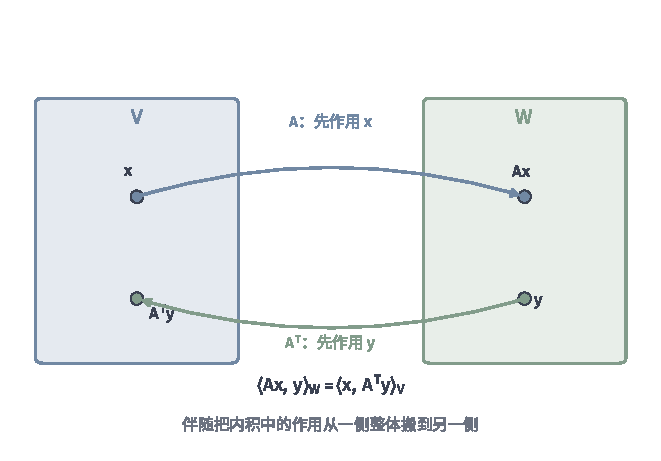
\includegraphics[width=112mm]{figures/01-mathematical-preliminaries-upper/02-linear-spaces/matplotlib/ls-adjoint-action-transfer/ls-adjoint-action-transfer.pdf}
  \caption{内积伴随把输出端的配对搬回输入端。左：$T:V\to W$把$\bm x$映成$T\bm x$，与$\bm y\in W$配对；右：伴随$T^\star:W\to V$把$\bm y$映回$T^\star\bm y\in V$，使$\langle T\bm x,\bm y\rangle_W=\langle\bm x,T^\star\bm y\rangle_V$。标准欧氏内积下$T^\star$就是转置，是配对方向的反转而非逆作用。箭头与空间为解析示意。}
  \label{fig:ls-adjoint-action-transfer}
\end{figure}

\paragraph{自伴、正交与正规算子}
对算子$T:V\to V$，伴随仍是$V$上的算子，可以与$T$比较。若$T^\star=T$，称$T$为\term{自伴}（self-adjoint）算子，标准坐标下对应对称矩阵。若$Q^\star Q=\operatorname{id}$，则$Q$保持内积：$\langle Q\bm x,Q\bm y\rangle=\langle\bm x,Q^\star Q\bm y\rangle=\langle\bm x,\bm y\rangle$，称为正交算子；标准坐标下它对应第~\ref{sec:ls-orthogonal-matrices}节的正交矩阵，且由方阵的单侧逆即双侧逆，$Q^{-1}=Q^\star$。满足$TT^\star=T^\star T$的算子称为\term{正规}（normal）算子，自伴与正交都属于它。这些类别的谱性质在第~\ref{chap:linear-analysis}章展开，这里只给出定义。

\subsection{完备性与Hilbert空间}
\label{sec:ls-hilbert-spaces}

前面的结论都在有限维内积空间中证明，证明里反复用到有限的基：正交直和要解有限阶的Gram方程，标准正交展开是有限和。函数空间中的内积，例如$\int_a^bf(t)g(t)\,\mathrm dt$，所在的空间是无限维的。这时哪些结论仍然成立，需要补充什么条件？答案的核心是第~\ref{sec:ls-banach-spaces}节的完备性。

\paragraph{Hilbert空间}
内积诱导范数，所以内积空间是赋范空间，可以问它在诱导范数下是否完备。在内积诱导的范数下完备的内积空间称为\term{Hilbert空间}（Hilbert space，也译作希尔伯特空间）。Hilbert空间都是Banach空间；反过来不成立。
\begin{example}[反例：完备但不来自内积的范数]
\label{ex:ls-banach-not-hilbert}
给定：$\mathbb R^2$配备$\ell_\infty$范数。

验证：这是有限维赋范空间，由定理~\ref{thm:ls-finite-dimensional-complete}完备，是Banach空间。示例~\ref{ex:ls-l1-linf-not-inner-product}已经算出，$\bm x=\bm e_1$、$\bm y=\bm e_2$使平行四边形恒等式不成立：左边为$2$，右边为$4$。所以这个范数不来自任何内积。

结论：$(\mathbb R^2,\lVert\cdot\rVert_\infty)$是Banach空间，但不是Hilbert空间。
\end{example}
由定理~\ref{thm:ls-finite-dimensional-complete}，有限维内积空间都完备，因而都是Hilbert空间；本节前面的结论都是有限维Hilbert空间中的结论。

无限维的基本例子是$\ell^2$：满足$\sum_kx_k^2<\infty$的实数列，内积为
\[
 \langle\bm x,\bm y\rangle=\sum_{k=1}^\infty x_ky_k .
\]
这个级数绝对收敛：对每个$n$，由$\mathbb R^n$中的Cauchy--Schwarz不等式，$\sum_{k\leq n}|x_ky_k|\leq(\sum_kx_k^2)^{1/2}(\sum_ky_k^2)^{1/2}$，部分和有界。它诱导的范数正是$\ell^2$范数，可以证明$\ell^2$完备。只保留有限个非零项，同一个内积给出的空间就不再完备。
\begin{example}[反例：有限非零数列的空间不完备]
\label{ex:ls-finite-sequences-incomplete}
给定：只有有限个非零项的实数列组成的线性空间$F$，配备上面的内积；序列$\bm x^{(n)}=(1,\tfrac12,\ldots,\tfrac1n,0,0,\ldots)\in F$。

计算：对$m>n$，由$1/k^2<1/(k-1)-1/k$（$k\geq2$），
\[
 \lVert\bm x^{(m)}-\bm x^{(n)}\rVert_2^2=\sum_{k=n+1}^m\frac1{k^2}
 <\sum_{k=n+1}^m\Bigl(\frac1{k-1}-\frac1k\Bigr)=\frac1n-\frac1m<\frac1n,
\]
所以这是柯西列。若它在$F$中收敛到某个$\bm x$，由$|x^{(n)}_k-x_k|\leq\lVert\bm x^{(n)}-\bm x\rVert_2$，每个坐标都收敛，极限只能是$(1,\tfrac12,\tfrac13,\ldots)$；这个数列属于$\ell^2$，却有无穷多个非零项，不在$F$中。

结论：$F$中的柯西列$\bm x^{(n)}$在$F$中没有极限，$F$不完备。
\end{example}
函数空间中情形相同：$C[a,b]$配备内积$\int_a^bfg\,\mathrm dt$是内积空间但不完备，补全后得到平方可积函数空间$L^2[a,b]$，它的构造需要第~\ref{chap:measure-spaces}章的Lebesgue积分。

\paragraph{完备性的作用}
完备性在无限维中承担有限维里由“有限个坐标”承担的工作。以标准正交展开为例。设$\bm q_1,\bm q_2,\ldots$是Hilbert空间中的一列标准正交向量，$\bm x$是任一向量。对每个$n$，式~\eqref{eq:ls-orthonormal-projection}后面的不等式给出$\sum_{k\leq n}\langle\bm x,\bm q_k\rangle^2\leq\lVert\bm x\rVert^2$，所以
\[
 \sum_{k=1}^\infty\langle\bm x,\bm q_k\rangle^2\leq\lVert\bm x\rVert^2 ,
\]
称为Bessel不等式。部分和$\bm s_n=\sum_{k\leq n}\langle\bm x,\bm q_k\rangle\bm q_k$满足$\lVert\bm s_m-\bm s_n\rVert^2=\sum_{n<k\leq m}\langle\bm x,\bm q_k\rangle^2$（勾股定理），由Bessel不等式，它是柯西列；空间完备，于是无穷展开$\sum_k\langle\bm x,\bm q_k\rangle\bm q_k$收敛到空间中的某个向量。在不完备的空间中，这一步可能失败：极限存在于更大的空间里，却不在原空间中。展开的极限是否就是$\bm x$本身，还取决于这列向量是否“足够多”，这是第~\ref{chap:functional-analysis-and-approximation}章完备正交系的问题。

正交直和与Riesz表示也是如此。有限维中它们靠有限的基与Gram方程证明；在Hilbert空间中，对\emph{闭}子空间$U$仍有$V=U\oplus U^\perp$，每个连续线性泛函仍能表示为与某个向量的内积，证明改用完备性保证最近点存在。第~\ref{sec:ls-finite-dimensional-sequences}节说明有限维中子空间总是闭的、线性泛函总是连续的，所以这些附加条件在有限维中自动满足。这些推广及其在函数逼近中的应用在第~\ref{chap:functional-analysis-and-approximation}章展开。
